\section{Evaluation}
\label{s:eval}

\FYI{

# Ext4
-
- Score

# F2FS
- Score

# Fragmentation on FDP?

}

% Evaluation environment
\FYI{
# Host configuration

# Lines of code

}


%  Git workload
The Git aging benchmark\cite{conway:login17,senescence:fast17} can measure aging in a real-world environment that people commonly use.
Git is a distributed version control system that allows synchronization of source code changes.
It generates workloads by simulating developers working on collaborative projects using Git.
Experiments are conducted using the git pull command, which creates new source files, deletes old files, or modifies files. During this process, Git maintains its internal data structure, leading to filesystem aging.
To measure the extent of aging, multiple git pull commands can be executed, and latency can be measured through reads using grep.

% Setup

\begin{figure}[t]
    \centering
    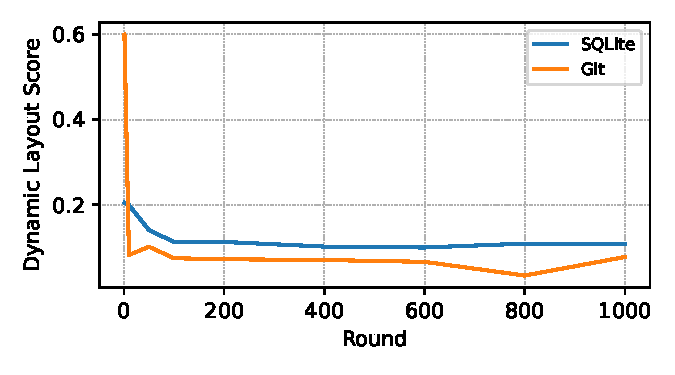
\includegraphics[width=0.95\columnwidth]{graphs/dynamic}
    \caption{Dynamic}
    \label{fig:dynamic}
\end{figure}

\begin{figure}[t]
    \centering
    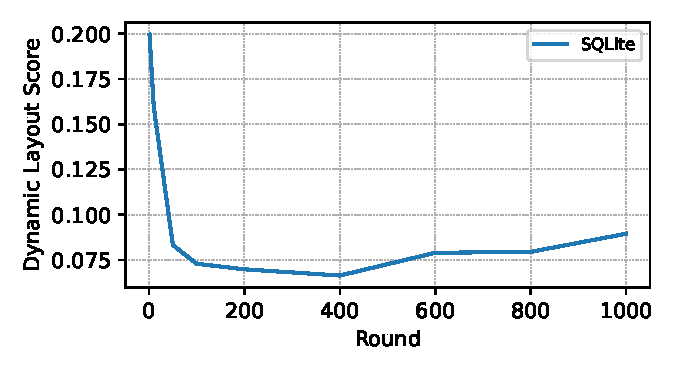
\includegraphics[width=0.95\columnwidth]{graphs/dynamic-f2fs}
    \caption{F2FS dynamic score}
    \label{fig:f2fs_dynamic_score}
\end{figure}


\begin{figure}[t]
    \centering
    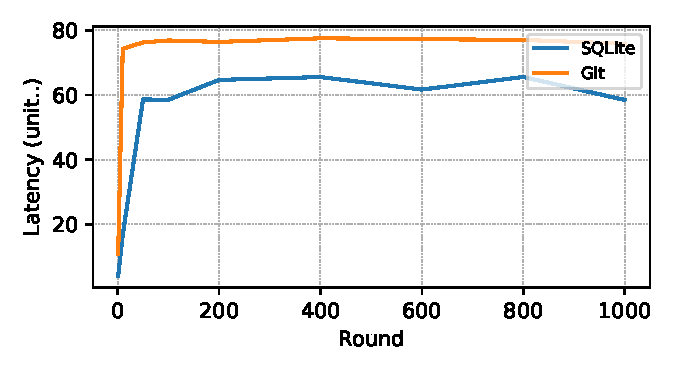
\includegraphics[width=0.95\columnwidth]{graphs/latency}
    \caption{Latency}
    \label{fig:latency}
\end{figure}

\begin{figure}[t]
    \centering
    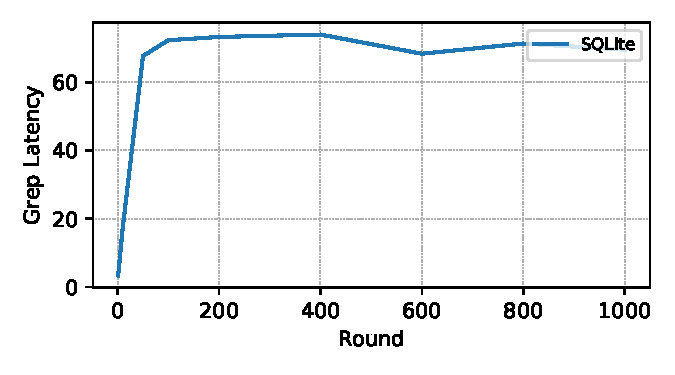
\includegraphics[width=0.95\columnwidth]{graphs/latency-f2fs}
    \caption{F2FS latency}
    \label{fig:f2fs_latency}
\end{figure}
